\documentclass[b5paper,11pt]{book}

\usepackage{geometry} 					% поля страницы

\usepackage{cmap}                       % Поддержка поиска русских слов в PDF (pdflatex)
\usepackage[T2A]{fontenc}				% Поддержка русских букв
\usepackage[utf8]{inputenc}            	% Выбор языка и кодировки
\usepackage[english, russian]{babel}	% Языки: русский, английский

\usepackage[unicode]{hyperref}			% Русский язык для оглавления pdf
\usepackage{bookmark}					% Оглавление в pdf
\usepackage{graphicx} 					% Подключаем пакет работы с графикой

\usepackage{amsmath,amssymb}

\usepackage{float}
\usepackage{subcaption}
\usepackage{algorithm}
\usepackage[noend]{algpseudocode}

\graphicspath{{../../images/textbooks/}} 			% Пути к изображениям

\geometry{left=2cm,right=2cm,top=2cm,bottom=2cm}	% Геомтерия страницы

\usepackage[
%	autolang=hyphen,
language=auto,
autolang=other,
backend=biber,
style=gost-numeric
]{biblatex}
\addbibresource{ids.bib}

\DeclareSourcemap{
	\maps[datatype=bibtex, overwrite]{
		\map{
			\step[fieldset=langid, fieldvalue=english]
			\step[fieldset=doi, null]
			\step[fieldset=issn, null]
			\step[fieldset=isbn, null]
			\step[fieldset=url, null]
			\step[fieldsource=language, fieldset=langid, origfieldval]
		}
	}
}

\newtheorem{Def}{Определение}
\newtheorem{Th}{Теорема}
\newtheorem{St}{Утверждение}

\numberwithin{Def}{section}
\numberwithin{Th}{chapter}
\numberwithin{St}{chapter}

\floatname{algorithm}{Алгоритм}
\algrenewcommand\algorithmicrequire{\textbf{Вход:}}
\algrenewcommand\algorithmicensure{\textbf{Выход:}}
\algrenewcommand\algorithmicforall{\textbf{для всех}}
\algrenewcommand\algorithmicwhile{\textbf{пока}}
\algrenewcommand\algorithmicif{\textbf{если}}
\algrenewcommand\algorithmicthen{\textbf{то}}
\algrenewcommand\algorithmicelse{\textbf{иначе}}
\algrenewcommand\algorithmicreturn{\textbf{вернуть}}
\algrenewcommand\algorithmicfunction{\textbf{функция}}
\algrenewcommand\algorithmicdo{}
\renewcommand{\algorithmiccomment}[1]{{\quad\sl // #1}}

\let\cleardoublepage\clearpage

\begin{document}
	\begin{titlepage}
		\begin{center}
			{\bfseries  Федеральное государственное автономное \\
				образовательное учреждение высшего образования\\
				<<Российский университет дружбы народов>>
				
			}

			\vspace{-5pt}
			\noindent\rule{\textwidth}{2pt}
			
			\vspace{50pt}
			{\Large\bfseries А.\,И.~Панов}
			
			\vspace{100pt}
			{\Huge\bfseries Интеллектуальные динамические системы}
			
			\vspace{20pt}
			{\Large\itshape Учебно-методическое пособие}
			
			\vfill
			{\bfseries Москва\\
				Российский университет дружбы народов\\
				2015
			}
		\end{center}
	\end{titlepage}
	
	\chapter*{}
	
	В пособии рассмотрены основные методы, применяющиеся при построении интеллектуальных динамических систем (ИДС). Одним из основных свойств ИДС является свойство иерархичности, уровневости организации всех процессов, связанных с ИДС, начиная от управления такими системами и заканчивая процессами самоорганизации в их базе знаний.
	
	
	\tableofcontents %% содержание
		
	\chapter*{Введение}
	\addcontentsline{toc}{chapter}{Введение}
	Динамические интеллектуальные системы "--- результат интеграции интеллектуальных систем с динамическими системами. В общем случае это двухуровневые динамические модели, где один из уровней отвечает за стратегию поведения системы (или, как иногда говорят, носит делиберативный характер), а другой уровень отвечает за реализацию конкретной (в том числе, математической) модели.
	
	К таким системам относятся сложные естественные системы, такие как экологические, социальные и политические системы, а также такие динамические системы, в которых зависимости настолько сложны, что не допускают своего обычного аналитического представления. Сложность задач управления, в которых существенная роль принадлежит экспертным суждениям и знаниям человека, заставляет в дополнение к количественным методам или вместо них применять такие подходы, в которых в качестве значений переменных допускаются не только числа, но и слова или предложения искусственного или естественного языка. 
	
	Потребность в моделях такого рода назрела в связи с развитием, например, беспилотных средств транспортного и иного назначения. В частности, в беспилотных автономных самолетах и вертолётах одним из уровней управления должен являться делиберативный уровень управления, решающий задачи, например, планирования полёта или выбора траектории или выбора цели. Другой уровень управления "--- назовем его активным "--- реализует требуемые действия. Например, на  делиберативном уровне управления беспилотным вертолётом принимается решение о зависании над целью, тогда на активном уровне начинает работать математическая модель зависания, вырабатывающая требуемые управления для исполнительных механизмов.
	
	\chapter{Представление статических знаний}
	
	\section{Логика предикатов первого порядка}
	Одним из наиболее изученных формальных языков является язык исчисления предикатов первого порядка. Существуют работы, где язык исчисления предикатов рассматривается как язык представления знаний, однако, это не главное его назначение и мы будем использовать его, главным образом, в качестве средства описания элементов конструкций других языков, более ориентированных на представление знаний. 
	
	Опишем вначале основные конструкции языка исчисления предикатов первого порядка и их интерпретацию в духе \cite{Klini1973,Keisler1977}.
	
	\subsection{Описание языка}\label{LangDescr}
	Основные конструкции языка $L$ – языка исчисления предикатов первого порядка называются формулами. Введем вначале \textit{алфавит} языка $L$. Алфавит включает:
	\begin{enumerate}
		\item Счетное множество букв: $z,y,x,\dots$, которое будем называть множеством символов для обозначения переменных языка.
		\item Счетное множество букв $a,b,c,\dots$, которое будем называть множеством символов для обозначения констант языка.
		\item Счетное множество прописных букв $P,Q,\dots$ для обозначения предикатных символов языка.
		\item Счетное множество строчных букв $f,g,\dots$ для обозначения функциональных символов.
		\item Символы для логических связок $\rightarrow$ (влечет), $\neg$ (не).
		\item Символ для квантора $\forall$ (для любого);
		\item (,) "--- скобки.
	\end{enumerate}
	
	Предикатные буквы $P,Q,\dots$ и функциональные буквы $f,g,\dots$ могут быть $n$-местными или, как еще говорят, $n$-арными. Иначе говоря, с каждым предикатным или функциональным символом будем связывать некоторое натуральное число, равное числу его аргументов.
	
	Определим теперь понятие формулы или правильно построенного выражения языка исчисления предикатов первого порядка. \textit{Формулы} языка определяются индуктивным образом. Начнем с определения \textit{терма} языка:
	\begin{enumerate}
		\item Переменная есть терм.
		\item Константа есть терм.
		\item Если $t_1,t_2,\dots,t_m,\dots,t_n$ "--- термы, а $f$ и $g$ "--- функциональные символы арности $m$ и $n$, соответственно, то  $f(t_1,t_2,\dots,t_m)$ и $g(t_1,t_2,\dots,t_n)$ также термы.
		\item Если $t_1,t_2,\dots,t_m,\dots,t_n$ "--- термы, а $P$ и $Q$ "--- предикатные символы арности $m$ и $n$, соответственно, то $P(t_1,t_2,\dots,t_m)$ и $Q(t_1,t_2,\dots,t_n)$ "--- атомарные формулы.
		\item Атомарная формула есть формула.
		\item Если $A,B$ "--- формулы, то $(A\rightarrow B)$, $\neg A$, $\neg B$ "--- формулы.
		\item Если $A$ "--- формула, то $\forall x A$ "--- формула.
		\item Всякое слово в алфавите языка является формулой тогда и только тогда, когда это можно показать с помощью конечного числа применений п.п. 1-7.
	\end{enumerate}

	Таким образом, мы завершили одно из возможных определений языка исчисления предикатов первого порядка. Существуют и другие определения, однако, язык, определенный нами, является полным, т.~е. в нем выразимо все то, что выразимо в языках (исчисления предикатов первого порядка), определенных любым иным способом.
	
	Можно, например, определить логические связки $\wedge, \vee$(читается \textit{и} и \textit{или}), выразив их через связки $\rightarrow$ и $\neg$:
	\begin{itemize}
		\item $A\wedge B = \neg(A\rightarrow\neg B)$,
		\item $A\vee B =\neg A\rightarrow B$.
	\end{itemize}
	
	Квантор существования "--- $\exists$ (существует) также выражается через квантор всеобщности и отрицание: $\exists x A(x) = \neg\forall x\neg A(x)$.
	
	Разумеется, $\wedge$, $\vee$ и $\exists$ с тем же успехом можно было бы включить в язык в качестве трех дополнительных символов. Есть, однако, некоторые преимущества в том, чтобы сохранить список символов как можно более коротким. Например, индуктивные определения и доказательства по индукции оказываются в этом случае короче.
	
	В дальнейшем нам придется использовать понятия \textit{свободного} и \textit{связанного} вхождения переменной в формулу. Вхождение переменной $x$ в формулу $A$ называется связанным, если эта переменная следует за квантором существования или всеобщности, предшествующими  формуле $A$. В противном случае, вхождение переменной называется свободным. Если в формуле $A$ отсутствуют свободно входящие в нее переменные (т.~е. либо все переменные связаны, либо просто отсутствуют), то формула называется \textit{замкнутой формулой} или \textit{предложением}. Атомарную замкнутую формулу будем называть \textit{фактом}. В том случае, если язык состоит только лишь из предложений, то он называется пропозициональным языком, а буквы $A,B,\dots$, входящие в формулы этого языка "--- пропозициональными переменными.
	
	\subsection{Основные понятия исчисления}\label{LangAx}
	Рассмотрим вкратце основные понятия исчисления предикатов первого порядка.
	
	Введем вначале аксиомы исчисления предикатов:
	\begin{enumerate}
		\item\label{ax1} $A\rightarrow (B\rightarrow A)$,
		\item\label{ax2} $(A\rightarrow (B\rightarrow C))\rightarrow ((A\rightarrow B)\rightarrow(A\rightarrow C))$,
		\item\label{ax3} $(\neg A\rightarrow \neg B)\rightarrow(B\rightarrow A)$.
	\end{enumerate}  
	А затем правила вывода:
	\begin{description}
		\item[Правило отделения:] если выводимо $A$ и выводимо $A\rightarrow B$, то выводимо $B$.
		\item[Правило подстановки:] в любую аксиому на место любой пропозициональной переменной можно подставить любое предложение, предварительно переименовав пропозициональные переменные подставляемого предложения так, чтобы они не совпадали с пропозициональными переменными аксиомы.
	\end{description}
	
	Если в аксиомах \ref{ax1} -- \ref{ax3} все переменные являются пропозициональными, то такое исчисление называется \textit{пропозициональным исчислением} или \textit{исчислением высказываний}.
	
	Рассмотрим пример вывода в исчислении высказываний. Возьмем, например, три закона логики, сформулированные Аристотелем и называемые постулатами Аристотеля. В языке исчисления высказываний они записываются следующим образом: 
	Пусть $P$ "--- пропозициональная переменная исчисления высказываний.
	\begin{description}
		\item[Постулат 1 (закон тождества):] $P\rightarrow P$.
		\item[Постулат 2 (закон исключения третьего):] $P\vee\neg P$.
		\item[Постулат 3 (закон противоречия):] $\neg(P\wedge\neg P)$.
	\end{description}
	
	Докажем один из постулатов, например закон тождества. Используем  аксиому \ref{ax1} и правило подстановки (вместо $B$ подставим $P\rightarrow P$) и получим $A\rightarrow((P\rightarrow P)\rightarrow A)$. Из аксиомы \ref{ax2}:
	\[
		(A\rightarrow((P\rightarrow P)\rightarrow C))\rightarrow((A\rightarrow(P\rightarrow P))\rightarrow(A\rightarrow C)).
	\]
	Теперь вместо $A$ и $C$ подставим $P$:  
	\[
		\underbrace{(P\rightarrow((P\rightarrow P)\rightarrow P))}_{X}\rightarrow\underbrace{((P\rightarrow(P\rightarrow P))\rightarrow(P\rightarrow P))}_{Y}.
	\]
	Затем применим правило отделения: та часть последней формулы, которая обозначена через $X$ является аксиомой, т.~е. выводима, тогда в силу правила отделения, выводима формула, обозначенная через $Y$. Теперь применим правило отделения к $Y$: 
	\[
		\underbrace{(P\rightarrow(P\rightarrow P))}_{X'}\underbrace{\rightarrow(P\rightarrow P)}_{Y'}.
	\]
	и, рассуждая таким же образом, получим, что $Y’$ "--- выводимо. Таким образом, закон тождества Аристотеля является \textit{теоремой} исчисления высказываний. Действуя таким же образом, можно доказать, что второй и третий постулаты Аристотеля также являются \textit{теоремами} исчисления высказываний.
	
	Однако, исчисление предикатов первого порядка не исчерпывается приведенными выше тремя аксиомами и правилами вывода. Смысл кванторов устанавливается еще двумя аксиомами и одним правилом вывода.
	\begin{enumerate}
		\setcounter{enumi}{4}
		\item\label{ax4} $\forall x((A\rightarrow B)\rightarrow(A\rightarrow\forall x B))$, где $x$ не является свободной переменной в $A$;
		\item\label{ax5} $\forall t A(t)\rightarrow A(x)$, где $t$ "--- терм, а $x$ не содержится в $t$ в качестве свободной переменной.
	\end{enumerate}
	Четвертая аксиома называется аксиомой генерализации, а вторая "--- аксиомой спецификации.
	
	\begin{description}
		\item[Правило обобщения:] $A\rightarrow\forall xA$, где $x$ "--- свободная переменная в $A$.
	\end{description}

	Аксиомы \ref{ax1}--\ref{ax5} исчисления предикатов первого порядка (или математической логики первого порядка) называются \textit{логическими} аксиомами, они описывают логические законы, справедливые всегда, независимо от предметной области. Если же к аксиомам \ref{ax1}--\ref{ax5} добавить еще и аксиомы, описывающие некоторую предметную область, например, арифметику или теорию групп, то получим \textit{формальную теорию} "---  формальную арифметику или формальную теорию групп, соответственно. При этом, разумеется, в алфавит языка следует ввести специальные функциональные символы, такие как сложение в арифметике или умножение в теории групп.
	
	Словосочетание <<первый порядок>> относится исключительно к тому обстоятельству, что кванторы $\forall$ и $\exists$ действуют на некотором универсальном множестве $U$. Логика второго порядка разрешает одному из кванторов действовать на подмножествах множества $U$ и на функциях из степеней $U$ в $U$. Логика третьего порядка может использовать кванторы по множествам функций и т.\,д. Уже из этих разъяснений видно, что в логиках более высоких порядков (как говорят, более сильных логиках) используются и некоторые нелогические понятия, такие как множество.
	
	\subsection{Формальные системы и интпретация}
	Будем полагать, что если заданы некоторый алфавит, множество формул, множества аксиом  и правил вывода, тотем самым задана некоторая формальная система. Иначе говоря, формальная система $F$ представляет собой совокупность следующих объектов:
	\[
		F=\langle T, P, A, \Pi\rangle,
	\]
	где $T$ "--- конечное множество символов; $P$ "--- множество правил грамматики, применение которых к символам из $T$, позволяет строить правильно построенные формулы; $А$ "--- множество аксиом;	$\Pi$ "--- множество правил вывода. 
	
	Если среди аксиом имеются нелогические аксиомы (аксиомы, описывающие некоторую предметную область), то формальная система называется \textit{формальной теорией}.
	\begin{Def}
		\textit{Выводом} (или \textit{доказательством}) в формальной системе называется конечная последовательность правильно построенных формул 
		\[
			A_1,A_2,\dots,A_n,
		\] таких что каждая из формул последовательности либо является аксиомой либо получена из предыдущих формул последовательности с использованием аксиом и правил вывода.
	\end{Def}
	
	Формула $A_n$ в этом случае называется \textit{выводимой формулой} (или \textit{теоремой}) формальной системы $F$.
	
	Введем теперь некоторые алгебраические понятия, которые окажутся полезными в дальнейшем.
	
	\begin{Def}
		$n$-арным отношением $R$ на $М$ называется подмножество $M^n$ и записывается как $R\subset M^n$.
	\end{Def}
	
	Пусть задано непустое множество "--- \textit{универсум} $M$. Дадим следующее определение, следуя \cite{Maltcev1970}.
	
	\begin{Def}
		Упорядоченную тройку  $S=\langle M, G, R\rangle$, где универсум $М$ называется основным множеством, $G$ "--- множество $n$-местных функций из $M^n$ в $M$, а $R$ "--- семейство $n$-арных отношений на $M$, будем называть алгебраической системой. 
	\end{Def}
	Если в определении алгебраической системы $S$ положить $R=\emptyset$, то такая алгебраическая система называется \textit{алгеброй}, а если $G=\emptyset$, то тогда алгебраическая система называется \textit{моделью}. 
	
	Иногда удобнее использовать  понятие \textit{многосортной} или \textit{многоосновной} алгебраической системы, полагая  существование нескольких основных множеств $M_1,M_2,\dots,M_n$, вместо одного множества $М$. Тогда функции из $G$ и отношения из $R$ становятся многосортными, т.~е. с каждым местом в списке аргументов функции или отношения связывается  некоторый сорт $i$, задаваемый, например, индексом одного из множеств из $M_i$ ($i=1,2,\dots,n$), а сами функции и отношения определяются на декартовых произведениях множеств из числа основных множеств.
	
	Пусть заданы формальная система $F$ с языком $L$ и алгебраическая система $S$. Определим  отображение $I$, которое всякому константному символу $a$ языка $L$ системы $F$ ставит в соответствие некоторый элемент $m\in M$ из алгебраической системы $S$, всякому $n$-местному предикатному символу $P$ "--- $n$-местное отношение $R\subset M^n$, а всякому $m$-местному функциональному символу $f$ "--- $m$-местную функцию $G:M^n\rightarrow M$. Тогда $I$ называется \textit{интерпретирующим отображением}, а  алгебраическая система $S$ "--- \textit{моделью} или \textit{интерпретацией} формальной системы $F$. Элементы множества $М$, функции и отношения, соответствующие константным, функциональным и предикатным символам языка $L$ в смысле отображения $I$, называют иногда интерпретациями константных, функциональных и предикатных  символов языка $L$, соответственно.
	
	Если интересоваться в большей степени собственно языком, нежели фактами, которые на нем записаны, то можно говорить и о моделях языка. Моделью $\Omega$ языка $L$ называется  пара $\langle M, I\rangle$, где $М$ и $I$ уже использовавшиеся только что универсум и интерпретирующее отображение. Заметим, что при данном универсуме $М$ для символов языка $L$ существует много различных интерпретаций.
	
	\subsection{Истинность в модели}
	Рассмотрим теперь вопрос об истинности или ложности формул языка $L$ в некотором возможном мире, т.~е. в модели. 
	
	В полной мере этот вопрос  оказывается не таким уж простым.	Например, не существует регулярного метода, позволяющего по произвольной формуле языка $L$ решать, истинна она или ложна в алгебраической системе $\langle N, +, *,\sigma, 0\rangle$, где $N$ "--- множество целых чисел, $+$, $*$ и $\sigma$ "--- операции сложения, умножения чисел и получения следующего числа, соответственно; 0 – константа нуль (которую можно рассматривать как нульместную функцию). Заметим попутно, что эта алгебраическая  система называется стандартной моделью арифметики.
	
	Чтобы определить понятие <<Предложение (формула) $A$ истинно в модели $\Omega$>>, мы должны вначале разбить $A$ на меньшие части и решить это вопрос для каждой из полученных частей. Если $А$ имеет вид  $\neg В$ или $В\wedge С$, то ясно, что вначале надо решить вопрос об истинности $В$ и $С$. С другой стороны, если $А$ имеет вид $\forall x B$, то такое рассуждение не проходит, так как $B$ может и не быть предложением, поэтому бессмысленно спрашивать,  истинно $В$ в $\Omega$ или ложно. На самом деле, предполагается, что значения всякой свободной в формуле $B$ переменной пробегают множество $M$. Поэтому, имеет смысл вопрос: является ли формула $B$ истинной в модели $\Omega$, если значением  свободной переменной является $m$? Если для каждого $m$ из $M$ ответ на этот вопрос окажется утвердительным, то можно говорить, что $A$ истинно в $\Omega$. Если же в $M$ найдется элемент $m$, для которого ответ будет отрицательным, то будем говорить, что $A$ ложно в $\Omega$. Однако, если $B$ имеет вид $\forall y C$, придется вновь преодолевать те же трудности. Поэтому, определение истинности формул в модели является  индуктивной процедурой, основанной на индуктивном определении формулы языка $L$ из раздела \ref{LangDescr}.
	
	Напомним что, интерпретирующее отображение $I$ всякому константному символу $a$ языка $L$  ставит в соответствие некоторый элемент $m\in M$, всякому $n$-местному предикатному символу $P$ "--- $n$-местное отношение $R\subset M^n$, а всякому $m$-местному функциональному символу $f$ "--- $m$-местную функцию $G:M^m\rightarrow M$; иначе говоря,  $I(a)=m$, $I(P)=R$ и $I(f)=G$, соответственно. 
	
	Итак, пусть, $P$ "--- $n$-местный предикатный символ, $x_1,x_2,\dots,x_n$ "--- свободные переменные. Будем говорить, что:
	\begin{enumerate}
		\item\label{true_1} Атомарная формула  $P(x_1,x_2,\dots,x_n)$ выполняется на $n$-ке $(I(a_1), I(a_2),\dots, I(a_n))$ в  модели $\Omega$, если $(I(a_1),I(a_2),\dots,I(a_n))\in I(P)$.
		\item Формула $\forall x_1 \forall x_2 \dots \forall x_n P(x_1,x_2,\dots,x_n)$ истина в модели $\Omega$, если формула $P(x_1,x_2,\dots,x_n)$ выполняется на любой $n$-ке $(m_1,m_2,\dots,m_n)\in I(P)$. Заметим, что если $a_1,a_2,\dots,a_n$ "--- константы, то для атомарной формулы $P(a_1,a_2,\dots,a_n)$ понятия выполнимости и истинности в модели $\Omega$ эквивалентны.
		\item Формула $\neg A$ истинна в модели $\Omega$, если $A$ "--- ложна.
		\item\label{true_4} Формула $A\rightarrow B$ истинна в модели $\Omega$, если $A$ "--- истинна и $B$ "--- истинна, либо $A$ "--- ложна и $B$ "--- ложна, либо $A$ "--- ложна, а $B$ "--- истинна (в модели $\Omega$).
		\item Формула может быть истиной только в силу п.п. \ref{true_1}--\ref{true_4}.
	\end{enumerate}
	
	В случае, когда $A$ не истина в $\Omega$, мы говорим, что $A$ ложна в $\Omega$, или что $A$ не выполняется в $\Omega$, или что $\Omega$ "--- модель предложения $\neg A$. Если дано множество предложений $\Sigma$, такое, что $\Omega$ является моделью каждого из предложений $\sigma\in\Sigma$, то $\Omega$ "--- модель этого множества. Предложение, истинное в каждой модели языка $L$, называется истинным.
	
	Рассмотрим простой пример. Пусть в языке $L$ определен трехместный предикатный символ <<СЕМЬЯ>>. Интерпретирующее отображение $I$ таково, что ставит в соответствие этому предикатному символу трехместное отношение <<\textbf{СЕМЬЯ}>>. Т.е. I(<<СЕМЬЯ>>)=<<\textbf{СЕМЬЯ}>>. Поскольку это отношение (как и всякая семья) конечно, то можно задать его в виде таблицы, каждая строка которой содержит имена членов одной семьи:
	
	\begin{table}[H]
		\centering
		\begin{tabular}{|c|c|c|}
			\hline
			\textbf{Мать} & \textbf{Отец} & \textbf{Ребенок}\\
			\hline
			Аня & Петя & Вася\\
			\hline
			Галя& Женя & Коля\\
			\hline
		\end{tabular}
	\end{table}
	
	Тогда модель включает универсум $M$, состоящий из имен членов всех семей и трехместное отношение <<\textbf{СЕМЬЯ}>>. Если мы желаем узнать что-либо о выполнимости формулы <<СЕМЬЯ>>($x,y,z$) в построенной таким образом модели, то, рассматривая различные наборы значений (из универсума $M$) переменных $x,y,z$, увидим, что в таблице имеется, например, строка (Аня, Петя, Вася). И отсутствует строка (Аня, Петя, Коля). Это означает, что формула <<СЕМЬЯ>>($x,y,z$) выполнима  в построенной модели, а именно, выполняется на тройках (Аня, Петя, Вася) и (Галя, Женя, Коля) и не выполняется, например, на тройке (Аня, Петя, Коля). Отсюда следует, в частности, что предложение $\forall x\forall y\forall z$<<СЕМЬЯ>>($x,y,z$) ложно, а, к примеру, предложение $\exists x\exists y \exists z$<<СЕМЬЯ>>($x,y,z$) истинно в построенной модели,
	
	Завершая этот раздел, вспомним о том, что язык $L$ "--- язык исчисления предикатов первого порядка и на нем записаны аксиомы этого исчисления, а для формул этого языка определены правила вывода и на них распространяется понятие выводимости (раздел \ref{LangAx}). Одно из основных утверждений, устанавливающих тесную связь между понятиями выводимости в исчислении предикатов первого порядка и истинности приведено ниже. 
	
	\begin{Th}[Гёделя о полноте]
		Произвольное предложение языка $L$ выводимо в исчислении предикатов первого порядка тогда и только тогда, когда оно истинно.
	\end{Th}
	
	\section{Атрибутивная логика}
	\section{Семантические сети}
	


	\chapter{Представление процедурных знаний}
	
	\section{Системы правил}\label{sect_rules}
	\section{Семиотическое представление}
	


	\chapter{Пополнение знаний}
	
	\section{Проблема привязки символов}
	\section{Биологически правдоподобные методы}
	\section{Выявление причинно-следственных связей}
	
	
	
	\chapter{Планирование поведения}
	
	\section{Классические алгоритмы планирования}
	\subsection{Планирование как доказательство теорем}
	
	Одним из примеров системы доказательства теорем, использовавшейся для решения задачи планирования, является система QA3 [53]. В системе QA3 одно множество утверждений используется для описания начального состояния, а другое "--- для описания эффектов действий. Чтобы следить за тем, какие факты являются истинными и в каком состоянии, в каждый предикат включаются выделенные переменные состояния. Целевое условие описываются формулой с переменной, связанной квантором существования. Задача системы состоит в том, чтобы доказать существование состояния, в котором истинно целевое условие. В основе доказательства лежит метод резолюций.

	Эксплуатация QA3 продемонстрировала её низкую вычислительную эффективность.	Кроме того, для неё не существовало сколько-нибудь приемлемого решения \textit{проблемы фрейма}. Суть этой проблемы состоит в том, что действие может иметь нелокальный эффект, иначе говоря, неясно какие формулы, описывающие состояние системы, изменяются при применении действия. Это, приводит к тому, что в описание действия включаются утверждения об изменении (не изменении) каждого факта, представленного в состоянии. Очевидно, что в сложных предметных областях описание эффектов действий значительно усложняется. 
	
	\subsection{Планирование в пространстве состояний}
	
	Первым планировщиком, осуществляющим планирование в пространстве состояний, является STRIPS (STanford Research Institute Problem Solver).STRIPS изначально разрабатывался для решения задачи формирования плана поведения робота, перемещающего предметы через множество помещений.
	
	Собственно, идея алгоритма STRIPS заимствована из системы GPS [55]. Метод, использованный в GPS, назывался анализ средств и целей (means-ends analysis). Он подразумевает рассмотрение в текущем состоянии тех действий, которые имеют отношение к цели. Однако, при таком подходе возникает следующая проблема: применять ли действия, связанные с целью, немедленно, как только они найдены или же приостановить применение действия до тех пор, пока не будут найдены все действия имеющие отношение к цели? STRIPS применяет действия не откладывая, достигая каждой цели по отдельности.
	
	МакДермот показал, что эффективность планирования с использованием метода анализа средств и целей может быть намного повышена задержкой применения действия до тех пор, пока не будут найдены все релевантные (относящиеся к цели действия) и повторением поиска релевантных действий заново, после каждого применения действия.	Для решения проблемы фрейма STRIPS предлагает в состоянии, к которому применяется правило (действие), изменять выполнимость лишь тех формул, которые описаны в эффекте действия, а выполнимость всех остальных оставлять неизменной.
	
	Рассмотрим постановку задачи планирования при классических допущениях в терминах STRIPS.	Как и выше, фактом будем называть замкнутую атомарную формулу языка исчисления предикатов 1-го порядка (ИПП), а состоянием "--- некоторое множество фактов. Неформально, состояние представляет модель среды, в которой действует  интеллектуальный агент.
	Приведём пример описания среды в терминах STRIPS:
	
	\[
		s = \{ATR(a), AT(B,b), AT(C,c), \forall u\forall x\forall y ((AT(u,x) \wedge (x \not= y)) \rightarrow \neg AT(u,y))\}.
	\]
	Здесь, $ATR(a)$ означает, что <<робот находится в комнате $a$>>, $AT(B,b)$ "--- <<ящик $B$ находится в комнате $b$>>, $AT(C,c)$ "--- <<ящик $C$ находится в комнате $c$>>. Имена конкретных объектов из этого множества: $a$, $b$, $c$ "--- соответственно <<комната $a$>>, <<комната $b$>>, <<комната $c$>>; $A$, $B$, $C$ "--- соответственно, <<ящик $A$>>, <<ящик $B$>>, <<ящик $C$>>.
	
	Действия агента будем описывать с помощью правил, при этом, для упрощения таких описаний, примем некоторые соглашения. При описании STRIPS-задачи планирования как в множествах добавляемых, так и в множествах удаляемых фактов будем использовать  лишь атомарные формулы без функциональных символов. Пример правила:
	
	\begin{table}[H]
		\centering
		\begin{tabular}{l c}
			Имя правила: & $Push(x, y, z)$\\
			Условие: & $C(R) = \{ATR (y), AT(x, y)\}$\\
			Список добавлений: & $A(R) = \{ATR (y), AT(x, y)\}$\\
			Список удалений: & $D(R) = \{ATR (z), AT(x, z)\}$
		\end{tabular}
	\end{table}
	
	В приведённом примере STRIPS-правило $Push(x, y, z)$ описывает действие робота по перемещению ящика $x$ из комнаты $y$ в комнату $z$. Здесь, $x$, $y$, $z$ "--- переменные. Выполнение агентом действия сводится к применению правила. Применение правила модифицирует состояние $s$.	Определение применимости правила было приведено в \autoref{sect_rules}. Применение правила $R$ преобразует состояние $s$ в $s'$ следующим образом:
	
	\[
		s' = (s \setminus (D(R)\theta)) \cup (A(R)\theta)).
	\]
	Это преобразование обозначается так: $s \overset{R,\theta}{\Rightarrow} s'$, где через $\theta$ обозначена подстановка элементов предметной области вместо переменных.
	
	\begin{Def}[STRIPS-допущение]
		При применении некоторого правила $R$ к состоянию $s$ выполнимость факта $f\in s$ изменяется, только если факт $f$ описан либо в списке удалений $D(R)$, либо в списке добавлений $A(R)$.
	\end{Def}
	
	Технически, при проверке применимости некоторого правила $R$, STRIPS выполняет полную подстановку на места всех переменных индивидов предметной области. Возможны различные варианты подстановок. Некоторые варианты подстановки могут давать примеры правил, применимых (или же неприменимых) в состоянии $s$. Однако, в алгоритм STRIPS можно внести незначительные модификации для применения не полностью означенных правил. В этом случае, в состоянии $s$ появились бы факты с переменными в описании. Как будет видно далее, неполная подстановка активно используется планировщиками в пространстве планов. Соответствующее свойство этих планировщиков получило название \textit{малого связывания} (least commitment).
	
	Приведем постановку задачи STRIPS-планирования.
	
	\begin{Def}
		Будем называть доменом планирования $P = \langle s_0, \Sigma R\rangle$, где $s_0$ "--- начальное состояние, $\Sigma R$ "--- конечное множество правил.
	\end{Def}
	\begin{Def}
		Будем называть задачей планирования $T = \angle P, G\rangle$, где $G$ "--- описание целевого факта агента, или просто цель.
	\end{Def}

	Решение задачи планирования $T$ заключается в нахождении плана, который достигает цели $G$.
	\begin{Def}
		План $Plan$ "--- это последовательность состояний $s_0,\dots,s_n$, последовательность правил $R_1,\dots,R_n$ и последовательность подстановок $\theta_1,\dots,\theta_n$, такая что, $G$ выполнима в $s_n$. Длина плана $Plan$ равна $n$:
		\[
			Plan: s_0 \overset{R_1,\theta_1}{\Rightarrow} s_1 \overset{R_2,\theta_2}{\Rightarrow} s_2 \dots \overset{R_n,\theta_n}{\Rightarrow} s_n.
		\]
	\end{Def}
	
	На вход алгоритма STRIPS подаётся множество правил $\Sigma R$, начальное состояние $s_0$, цель $G$.
	
	\begin{algorithm}[H]
		\caption{Алгоритм STRIPS}\label{alg:strips}
		\begin{algorithmic}[1]
			\Require $\Sigma R$, $s$, $G$
			\Ensure $Plan$
			
			\State $s=s_0$
			\While $G$ не выполнимо в $s$
				\State выбрать компоненту $g$ из $G$ \label{alg_st:goal}
				\State выбрать правило $R\in\Sigma R$ такое, что $g\in A(R)$ \label{alg_st:act}
				\State \Call{STRIPS}{$\Sigma R$,$s$,$C(R)$}
				\State применить $R$ к $s$ \label{alg_st:app}
				\State добавить $R$ в $Plan$
			\EndWhile
			
			\Return $Plan$
		\end{algorithmic}
	\end{algorithm}

	Будем полагать, что в множестве $\Sigma R$ все правила полностью конкретизированы. Вначале в стек целей помещается главная цель $G$. Если цель не является простой, т.~е. содержит конъюнкцию литералов, то система STRIPS добавляет в стек в некотором порядке каждый из литералов составной цели (шаг \autoref{alg_st:goal}). Когда верхняя цель стека является однолитеральной, система ищет действие (шаг \autoref{alg_st:act}), которое содержит в списке добавлений литерал, сопоставимый с этой целью. Если такое действие не применимо к текущему состоянию, тогда его предусловие помещается в стек целей, иначе действие применяется к текущему состоянию (шаг \autoref{alg_st:app}) и помещается в план $Plan$. Если верхняя цель в стеке соответствует текущему состоянию, то она удаляется из стека. Алгоритм STRIPS завершается, когда стек пуст.
	
	Существуют задачи, для которых STRIPS либо не может построить план, либо находит не минимальный план. Причина этого кроется в том, что STRIPS удовлетворяет каждую компоненту составной цели по отдельности, без учёта их взаимосвязи. Особенность предметной области, где цели взаимосвязаны (взаимодействуют) получила название взаимосвязи целей.
	
	\section{Планирование с удовлетворением ограничений}
	
	В этом разделе рассмотрим алгоритм планирования "--- Graphplan, который использует технику прямого распространения ограничений \cite{Blum1997}. В свое время (1997) Graphplan продемонстрировал хорошие результаты для ряда тестовых задач классического планирования. Создатели Graphplan'а объясняют этот успех способностью Graphplan'а анализировать множество планов одновременно. 
	
	Graphplan оказал сильное влияние на последующие работы в области планирования. Он принимает на вход стандартное STRIPS-описание задачи планирования и переводит это описание в компактную структуру, которая называется графом планирования, из которой впоследствии извлекает частично-упорядоченный план. Важно отметить, что граф планирования это не граф состояний, который получается при работе планировщика в пространстве состояний. Graphplan сочетает в себе свойства как планировщика в пространстве состояний, так и планировщика в пространстве планов. Иначе говоря, он не обладает свойством малого связывания. Приведем определения основных понятий планировщика.
	
	\begin{Def}
		Факты $F$ "--- множество элементарных формул без переменных из домена планирования $P$.
	\end{Def}
	
	Перед основной стадией работы Graphplan создаёт множество действий, осуществляя для каждого правила $R\in\Sigma R$ всевозможные варианты подстановки индивидов на места всех переменных. Имеется также специальный вид действия <<no-op>> "--- <<ничего не делать>>.
	
	\begin{Def}
		Действия $Acts$ "--- множество полностью конкретизированных правил из $\Sigma R$, а также действие <<no-op>>.
	\end{Def}

	Действие <<no-op>> имеет условие $C(\text{no-op})=f$, список добавлений $A(\text{no-op})=f$, и пустой список удалений $D(\text{no-op})=\emptyset$, где $f$ "--- произвольный факт из $F$.

	\begin{Def}
		Граф планирования $PG$ "--- ориентированный ярусный граф с двумя типами узлов и с тремя типами рёбер.	Два типа узлов в $PG$ таковы: 
		\begin{itemize}
			\item $FN$ "--- множество узлов, ассоциированных с фактами $F$, и 
			\item $AN$ "--- множество узлов, ассоциированных с действиями $Acts$.
		\end{itemize}

		Ассоциацию некоторого факта $f\in F$ с узлом $fn\in PG$, будем обозначать как $fn\rightarrow f$. Ассоциацию некоторого действия $act\in Acts$ с узлом $an\in AN\subset PG$, будем обозначать как $an\rightarrow act$.
		
		Множество узлов PG разбито на не пересекающиеся подмножества 
		\[
			\langle FL_0, AL_0, FL_1, AL_1, \dots, AL_{n-1}, FL_n\rangle,
		\]
		где $FL$ "--- ярус, содержащий узлы-факты, $AL$ "--- ярус, содержащий узлы-действия, $FL_0$ содержит узлы-факты, соответствующие фактам начальной ситуации $S_0$.
		
	\end{Def}

	Конфликт "--- это отношение взаимоисключения между двумя узлами на одном ярусе. Существуют конфликты между действиями и между фактами.

	\begin{Def}
		Конфликты $MXF$ "--- отношения взаимоисключения между узлами-фактами $(fn_1, fn_2)$, где $fn_1, fn_2$ "--- узлы-факты, находящиеся на одном ярусе, такие, что: либо все действия на предыдущем ярусе, добавляющие факт $fn_1$, удаляют факт $fn_2$; либо все действия на предыдущем ярусе добавляющие факт $fn_2$, удаляют факт $fn_1$.
	\end{Def}
	
	\begin{Def}
		Конфликты $MXA$ "--- отношения взаимоисключения между узлами-действиями $(an_1, an_2)$, где $an_1, an_2$ "--- узлы-действия, находящиеся на одном ярусе, такие, что действие $an_1$ удаляет условие	или же эффект действия $an_2$, либо предусловие действия $an_1$ и предусловие действия $an_2$ состоят в конфликте $mxf\in MXF$.
	\end{Def}

	Заметим, что конфликт между парой узлов $n_1$ и $n_2$, может иметь место на некотором ярусе $L$ и не иметь места на некотором последующем ярусе $L'$. С другой стороны, если между парой узлов $n_1$ и $n_2$ на некотором ярусе $L$ не существует конфликта, то и на последующих ярусах после $L$, пара узлов $n_1$ и $n_2$ не будет конфликтовать.
	
	Конфликты превращают граф планирования в граф ограничений в смысле CSP-задачи. Метод, который используется для построения графа планирования, называется прямым распространением ограничений.
	
	Любой ярус $AL_i\in PG$ содержит узлы-действия $an\rightarrow act$, такие что $Nodes(C(act\leftarrow an))\in FL_i$ и не существует $fn_1,fn_2\in Nodes(C(act\leftarrow an))$ и $(fn_1, fn_2)\in MXF$, где $Nodes(C(act\rightarrow an))$ "--- узлы на ярусе $FL_i$, ассоциированные, с фактами из предусловия $C(act)$. Любой ярус фактов $FL_i\in PG$ ($i>0$) содержит узлы-факты $fn\rightarrow f$, такие что, для любого $an\in AL_{i-1}\in PG$ справедливо $(f\in D(act\leftarrow an)$ или $f\in A(act\leftarrow an))$.
	
	Рёбра устанавливаются между узлами, расположенными на ярусах. Три типа рёбер $PG$ таковы:
	\begin{itemize}
		\item ребро-предусловие "--- устанавливается между узлом-фактом $fn\rightarrow f$ на некотором ярусе $FL_i$ и узлом-действием $an\rightarrow act$ на ярусе $AL_i$, если факт $f\in C(act)$;
		\item ребро-добавление "--- устанавливается между узлом-действием $an\rightarrow act$ на некотором ярусе $AL_i$ и узлом-фактом $fn\rightarrow f$ на ярусе $FL_{i+1}$, если $f\in A(act)$;
		\item ребро-удаление "--- устанавливается между узлом-действием $an\rightarrow act$ на некотором ярусе $AL_i$ и узлом-фактом $fn\rightarrow f$ на ярусе $FL_{i+1}$, если $f\in D(act)$.
	\end{itemize}

	Из определения видно, что ярусы $PG$ чередуются так: ярус фактов $|$ ярус действий и т.~д. Первый ярус графа содержит факты, характеризующие начальное состояние. Ярусы в $PG$ от самого первого до последнего содержат: факты, истинные в момент времени 1, действия, возможные в момент времени 1, факты, истинные в момент времени 2, действия, возможные в момент времени 2 и т.д. По сути, граф планирования $PG$ позволяет представлять пространство состояний без разделения. Точнее, множество состояний хранящиеся совместно, например, на ярусе $FL_{j+1}$, получаются в результате всевозможных альтернативных вариантов применения действий, расположенных в ярусах $AL_i$ по $AL_j$ ($i<j$), к некоторому состоянию $s$, представленному на ярусе фактов $FL_i$. Однако, ясно, что альтернативная перестановка $k$ действий может привести к тому, что одно из действий может удалять эффект, либо условие другого действия. Для обработки подобных ситуаций используются так называемые  конфликты между действиями и конфликты между фактами. Это позволяет при необходимости, например, на этапе извлечения плана, выделить из графа $PG$ альтернативные компоненты пространства состояний. Планировщики, использующие такой способ представления пространства состояний, получили название \textit{дизъюнктивных планировщиков}. 
	
	\begin{Def}
		Пара ярусов фактов $FL_i$ и $FL_j$ "--- идентична, если $FL_i$ и $FL_j$ содержат одинаковые факты и одинаковые конфликты.
	\end{Def}
		
	\begin{Def}
		Граф Планирования $PG$ является стабилизированным, если существуют пара смежных ярусов фактов $FL_i$ и $FL_{i + 1}$ и $FL_i$ идентичен $FL_{i + 1}$.
	\end{Def}
	
	Справедливо следующее утверждение, которое мы приведем без доказательства.
	
	\begin{St}
		Пусть граф $PG$ стабилизирован, и имеется пара идентичных ярусов-фактов $FL_i, FL_{i + 1} \in PG$. Тогда, ярус фактов $FL_k\in PG$ идентичен ярусу фактов $FL_i\in PG$, где $k > i \in \mathbb{N}$.
	\end{St}
	
	Цель $G$ является разрешимой (достижимой) в следующих случаях: 
	\begin{itemize}
		\item если она удовлетворяется тривиальным образом, т. е. компоненты цели $G$ присутствуют в начальном ярусе фактов, 
		\item если в графе $PG$ существует подграф $Plan$, который состоит из множества путей, идущих от начального яруса
		фактов к ярусу фактов, содержащему $G$, и в этом множестве путей нет ни одной пары конфликтующих узлов.
	\end{itemize}
		
	\begin{algorithm}[h]
		\caption{Алгоритм GraphPlan}\label{alg:graphplan}
		\begin{algorithmic}[1]
			\Require $Acts, S_0, G$
			\Ensure $Plan$
			
			\State $t = 0$ \Comment{номер начальной стадии}
			\State $GS = \emptyset$ \Comment{множество для хранения разрешимых/неразрешимых целей}
			\State $PG.FL_0 \leftarrow S_0$
			\While{$PG$ не стабилизирован или цель $G$ не разрешима}
				\State \Call{SpreadGraph}{$PG$}
				\State \Call{SearchPlan}{$PG$}
				\State $t = t + 1$ \Comment{переход к следующей стадии}
			\EndWhile
			\If{<<цель $G$ разрешима>>}
				\State \Return $Plan$
			\Else
				\State \Return $Plan = \emptyset$
			\EndIf
		\end{algorithmic}
	\end{algorithm}

	\begin{algorithm}[h]
		\caption{Функция SpreadGraph}\label{alg:spread}
		\begin{algorithmic}[1]
			\Function{SpreadGraph}{$FL_t$}
				\Statex\Comment{создание следующего яруса действий $AL_{t + 1}$}
				\ForAll{действий $act\in ACTS$, применимых в $FL_t$}
					\If{для каждой пары фактов $f_1, f_2 \in C(act)$ не существуют узлы $fn_1\rightarrow f_1$, $fn_2 \rightarrow f_2$, такие что $fn_1, fn_2 \in FL_t$ и $fn_1, fn_2 \in mxf$}
						\State создать в $AL_{t + 1}$ узел-действие $an\rightarrow act$
						\State создать рёбра-предусловия между $an$ и соответствующими узлами $fn\in FL_t$
					\EndIf
				\EndFor
			
				\State выявить конфликты $mxa$ на ярусе $AL_{t + 1}$
				
				\Statex\Comment{создание следующего яруса фактов $FL_{t + 1}$}
				\ForAll{узлов $an\in AL_{t + 1}$}
					\State добавить в $FL_{t + 1}$ узлы-факты, ассоциированные с фактами из $A(act\leftarrow an)$ и $D(act\leftarrow an)$
					\State соединить соответствующими рёбрами добавления или рёбрами удаления узлы $FL_{t + 1}$ и узлы $AL_{t + 1}$
				\EndFor
				\State выявить конфликты $mxf$ на ярусе $FL_{t + 1}$
			\EndFunction
		\end{algorithmic}
	\end{algorithm}
	
	\begin{algorithm}[h]
		\caption{Функция SearchPlan}\label{alg:search}
		\begin{algorithmic}[1]
			\Function{SearchPlan}{}
				\Statex\Comment{результат: <<цель $G$ разрешима>>/<<цель $G$ пока не разрешима>>}
				\If{$GN \subseteq FL_t$}
					\State добавить $GN$ в $GS_i^t$, где $i$ "--- номер текущего яруса фактов, $t$	"--- номер текущей стадии, $GN$ "--- множество узлов-фактов, ассоциированных	с целевыми компонентами
				\EndIf
		
				\If{если \Call{CheckGoal}{$GS_i^t$}}
					\State \Return <<цель $G$ разрешима>>
				\Else
					\State \Return <<цель $G$ пока не разрешима>>
				\EndIf
			\EndFunction
		\end{algorithmic}
	\end{algorithm}
			
	\begin{algorithm}[h]
		\caption{Функция CheckGoal}\label{alg:checkgoal}
		\begin{algorithmic}[1]
			\Function{CheckGoal}{$GS_i^t$}
				\Statex\Comment{выход: <<$GS_i^t$ разрешимо>>/<<$GS_i^t$ не разрешимо>>}
				\Statex\Comment{$GS_i^t$ "--- множество (под)целей на $i$-ом ярусе фактов}
				\State $Comb$ "--- множество всех комбинаций $A_{comb}$ действий яруса $AL_{i-1}$ таких, что любая пара действий в $A_{comb}$ не состоит в конфликте $mxa \in MXA$, и при этом $A_{comb}$ доставляет $GS_i^t$
				\ForAll{$A_{comb} \subseteq Comb$} 
					\State создать подцель $GS_{i-1}^t$, состоящую из предусловий действий в $A_{comb}$
				\EndFor
				\If{цели $GS_{i-1}^t$ разрешимы}
					\State добавить тройку $\langle GS_{i-1}^t, A_{comb}, GS_i^t\rangle$ в $Plan$
					\State\Return <<$GS_i^t$ разрешимо>>
				\ElsIf{цели в $GS_i^t$ не разрешимы}
					\State\Return <<$GS_i^t$ не разрешимо>>
				\EndIf
			\EndFunction
		\end{algorithmic}
	\end{algorithm}
	
	Имеют место следующие утверждения: 
	\begin{itemize}
		\item план длиной $n$ можно извлечь из графа планирования $PG$, содержащего $n$ ярусов-действий;
		\item алгоритм GraphPlan возвращает <<план не существует>>, только если цель G не достижима;
		\item алгоритм GraphPlan обладает полнотой.
	\end{itemize}

	В начале Graphplan формирует первичный ярус фактов $FL_0$. Выполнение алгоритма включает ряд стадий (переменная $t$ в алгоритме). На каждой стадии выполняется расширение графа планирования $PG$ и поиск плана в графе $PG$.
	
	На этапе расширения графа $PG$ на основе текущего яруса фактов создаётся новый ярус действий, а затем, на основе нового яруса действий,	формируется новый ярус фактов. Во вновь сформированных ярусах выявляются конфликты $MXF$ и $MXA$ (процедура SpreadGraph).
	
	Graphplan строит частично-упорядоченный план. Извлечение плана осуществляется с помощью техники обратного хода от текущего яруса к начальному ярусу. Эта техника позволяет более эффективно использовать	информацию о конфликтах между действиями и фактами в графе $PG$. Опишем эту технику.
	
	Перед поиском плана Graphplan проверяет следующее условие: <<справедливо ли, что $GN\subseteq FL_{\text{тек}}$ и для каждой пары узлов $gn_1,gn_2\in GN$ и $gn_1,gn_2\not\in mxf$, где $GN$ "--- множество целевых фактов, ассоциированных с узлами на ярусе $FL_{\text{тек}}$>>. Если это так, тогда возможно план существует, и Graphplan приступает к поиску. Суть поиска плана сводится к тому, чтобы от целевых фактов в текущем ярусе $GN\subseteq FL_{\text{тек}}$, выделить путь, ведущий к ярусу $FL_0$. В пути не
	должны содержаться конфликтные действия. На основе выделенного пути	формируется план. Более точно происходит следующее: формируется множество $GS$ "--- хранилище (под)целевых наборов $GS_i^t$. $GS_i^t$ "--- множество целей, выбираемые из яруса фактов с номером $i$,
	при поиске плана на стадии $t$.
	
	Начиная с текущего яруса $FL_i$ (вначале $i = t$) в $GS_i^t$ заносятся целевые факты $GN\subseteq FL_i$. Далее на ярусе действий с номером $i-1$ выделяются всевозможные комбинации действий ($A_{comb}$), доставляющие $GS_i^t$ (множество $Comb$). Устанавливается подцель $GS_{i-1}^t$, в которую помещаются предусловия выделенных действий, расположенные на ярусе фактов $FL_{i-1}$. Для каждой из комбинаций действий $A_{comb}\subseteq Comb$ процесс продолжается рекурсивно, до тех пор, пока $GS_{i-1}^t$ окажется тривиально разрешимой, либо не найдётся комбинации действий, доставляющей $GS_{i-1}^t$, т.~е. $Comb = \emptyset$.
	
	Если подцель $GS_{i-1}^t$ оказывается разрешимой, то при возврате из рекурсии в план $Plan$ помещаются тройки $\langle GS_{i-1}^t, A_{comb}, GS_i^t\rangle$, в которой для каждого действия из $A_{comb}$, известно какие (под)цели из $GS_i^t$ достигает действие, и какие цели из $GS_{i-1}^t$ необходимо достичь, прежде чем выполнить действие. 
	
	Для получения линейного плана необходимо выполнить топологическую сортировку нелинейного плана $Plan$, с учётом целевых ограничений $GS_i^t$. При реализации алгоритма для повышения эффективности обратной техники извлечения плана, используется хеширование. В хеш-таблице на каждой стадии $t$ запоминаются целевые наборы $GS_i^t$, которые оказались не разрешимыми в ярусе фактов $i$. На каждой стадии при поиске плана проверяется наличие в хэш-таблице разрешаемой подцели $GS_{i-1}^t$. Если подцель $GS_{i-1}^t$ в хеш-таблице, то поиск плана немедленно прекращается, и исходная цель $GS_i^t$, также помещается в хеш, как неразрешимая.
	
	\section{Нелинейное планирование}

	Составление частично-упорядоченных планов рассмотрим на примере планировщика SNLP (Systematic Nonlinear Planning) \cite{McAllester1991}. 
	
	Учитывая, что план это последовательность операторов, очевидно, что два плана можно рассматривать как эквивалентные, если один из них может быть выведен из другого посредством	переупорядочивания невзаимодействующих шагов. Например, рассмотрим робота, который	должен выполнить набор задач в комнате $A$ и набор задач в комнате $B$. Каждая задача формально ассоциируется с конкретным целевым высказыванием. Мы хотим достичь (сделать истинными) высказывания $P_1, \dots, P_n, Q_1, \dots, Q_m$. У нас есть операторы $A_1, \dots, A_n, B_1, \dots, B_m$, где $A_i$ действие делает истинным $P_i$ высказывание и при этом должно выполняться в комнате $A$, а $B_i$ действие делает истинным $Q_i$ высказывание и должно выполняться в комнате $B$. Более
	формально, каждое $A_i$ имеет одно предусловие $IN(A)$, добавляет высказывание $P_i$ и не удаляет никаких высказываний. Каждое $B_i$ определяется подобным образом с предусловием $IN(B)$.
	
	Пусть у нас также есть оператор $GO(A)$ без предусловий со списком добавления $IN(A)$ и списком удаления $IN(B)$. У нас также есть и аналогичный оператор $GO(B)$. Множество целей	$\{P_1, \dots, P_n, Q_1, \dots, Q_m\}$ может быть достигнуто (независимо от начального состояния) посредством плана 
	\[
		GO(A), A_1, \dots, A_n, GO(B), B_1, \dots, B_m.
	\] 
	Очевидно, что порядок $A_i$ шагов и порядок $B_i$ шагов не имеет значения, при условии, что все $A_i$ шаги будут выполнены в комнате $A$, а все $B_i$ шаги в комнате $B$. Этот план следует рассматривать как эквивалентный плану $GO(A), A_n, \dots, A_1, GO(B), B_m, \dots, B_1$, в котором шаги $A_i$ и $B_i$ выполняются в обратном порядке. Каждый (линейный) план, который является решением данной проблемы планирования, может быть обобщен <<нелинейным планом>>, который поддерживает только частичный порядок на шагах	плана. Два линейных плана рассматриваются как эквивалентные, если они являются разными представлениями одного и того же нелинейного (частично-упорядоченного) плана (см. \autoref{fig:snlp_example}).
	
	\begin{figure}[h]
		\centering
		\begin{subfigure}[b]{0.45\textwidth}
			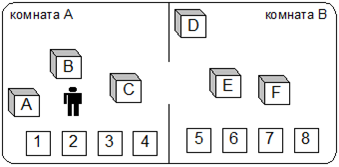
\includegraphics[width=\textwidth]{snlp_example.png}
			\caption{Пример частично-упорядоченного плана}
			\label{fig:snlp_example}
		\end{subfigure}
		\hfill
		\begin{subfigure}[b]{0.45\textwidth}
			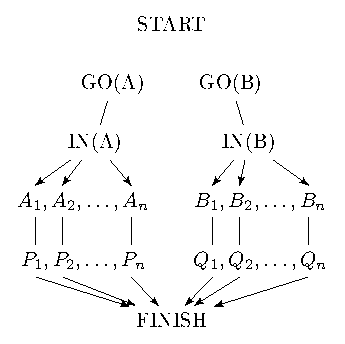
\includegraphics[width=\textwidth]{snlp}
			\caption {Причинные связи в линейном плане}
		\end{subfigure}
		\caption{Пример SNLP планирования}
		\label{fig:snlp_causal}
	\end{figure}
	
	Чтобы определить нелинейный план, связанный с данным линейным планом, мы сначала
	должны преодолеть небольшую техническую проблему. В линейном плане мы можем
	именовать отдельные шаги плана, ссылаясь на них, как на первый шаг, второй шаг и т.~д. Однако в нелинейном плане может не быть четко определенного второго шага. Мы также не можем именовать шаги именами операторов, используемых в этих шагах, т.~к. несколько шагов	могут использовать один и тот же оператор. Для именования шагов в нелинейном плане мы	будем полагать, что с каждым шагом ассоциировано отдельное символьное имя, которое	называется именем шага.
	
	\begin{Def}
		Таблица символов это отображение из конечного множества имен шагов в
		операторы. Каждая таблица символов должна содержать два особенных имени шага,
		называемых START и FINISH. START отображается на некий фиктивный оператор, который	не имеет предусловий и списка удалений, но добавляет множество <<начальных высказываний>>. Аналогично, FINISH отображается на оператор, который имеет множество предусловий, называемых <<целевыми формулами>>, но имеет пустые списки добавления и удаления.
	\end{Def} 
	
	\begin{Def}
		Причинная связь "--- это тройка $\langle S, f, W \rangle$, где $f$ "--- некоторый факт, $W$ "--- шаг, имеющий в предусловии факт $f$, $S$ "--- шаг, имеющий факт $f$ в списке добавлений.	
	\end{Def}

	\begin{Def}
		Угроза $V$ для причинной связи $\langle S, f, W\rangle$ "--- это шаг, который либо добавляет, либо удаляет факт $f$, и при этом не является ни шагом $S$, ни шагом $W$.		
	\end{Def}

	\begin{Def}
		Защитное ограничение "--- это отношение порядка $<$, заданное на шагах плана, при этом $S<W$ означает, что шаг $S$ должен быть выполнен до шага $W$, и наоборот, $S>W$ означает, что шаг $S$ должен быть выполнен после шага $W$.		
	\end{Def}

	\begin{Def}
		Нелинейный план $Plan = \langle ST, CL, SC\rangle$, где $ST$ "--- множество шагов, $CL$ "--- множество причинных связей, $SC$ "--- множество защитных ограничений.		
	\end{Def}

	Заметим, что нелинейный план $Plan$ обладает полнотой, если:
	\begin{itemize}
		\item каждый шаг плана участвует либо в причинной связи, либо в защитном ограничении;
		\item любой шаг $W$ с предусловием $f$ состоит в некоторой причинной связи $\langle S, f , W\rangle$;
		\item имеется шаг-угроза $V$ для причинной связи $\langle S, f, W\rangle$ и нелинейный план содержит либо защитное ограничение $V<S$, либо защитное ограничение $V>W$.
	\end{itemize}
		
	\begin{Def}
		Топологическая сортировка нелинейного плана $Plan$ "--- это линейная последовательность всех шагов, которая удовлетворяет следующим условиям:
		\begin{itemize}
			\item первый шаг в последовательности "--- START;
			\item последний шаг в последовательности "--- FINISH;
			\item для каждой причинной связи $\langle S, f, W\rangle$ шаг $S$ в последовательности предшествует шагу $W$;
			\item для каждого защитного ограничения $U<V$ шаг $U$ в последовательности предшествует шагу $V$.
		\end{itemize}
	\end{Def}

	Топологическая сортировка нелинейного плана является решением, если применение последовательности действий шагов между шагами START и FINISH из начального состояния, которое задаётся списком добавлений шага START, приводит в состояние, в котором содержатся все предусловия шага FINISH.
	
	\begin{Th} 
		Любая топологическая сортировка нелинейного плана, обладающего полнотой, является решением задачи планирования $T$.
	\end{Th}
	
	\begin{Def}
		Нелинейный план является противоречивым, если на нём невозможно осуществить топологическую сортировку.	
	\end{Def}
		 
	Таким образом, противоречивый нелинейный план не является решением задачи планирования.
	
	\begin{Th} 
		Алгоритм SNLP систематичен, т.~е. в процессе поиска, осуществляемого в пространстве частично-упорядоченных планов, один и тот же план или эквивалентные планы никогда не рассматриваются дважды.
	\end{Th}
	
	\begin{algorithm}[h]
		\caption{Алгоритм SNLP}\label{alg:snlp}
		\begin{algorithmic}[1]
			\Require $\sum R, Plan$
			\Ensure $Plan$, <<план построен>>/<<план не построен>>
			
			\If {$Plan$ противоречив}
				\State \Return $Plan=\emptyset$, <<план не построен>>
			\EndIf
			\If{$Plan$ обладает полнотой}
				\State \Return $Plan$, <<план построен>>
			\EndIf
			\If{в $Plan$ имеется шаг-угроза $V$ для причинной связи $\langle S,f,W\rangle$ и $Plan$ не содержит защитного ограничения $V<S$ или $V>W$}
				\State недетерминированно выполнить	
				\Statex (a) либо SNLP($Plan$+($V<S$)), 
				\Statex (b) либо SNLP($Plan$+($V>W$))
			\EndIf
			\If{существует некоторый шаг $W$ с предусловием $f$, для которого не существует причинной связи $\langle S,f,W\rangle$}
				\State недетермированно выполнить либо 
				\Statex (a) выбрать недетерминированно некоторый шаг $S$, добавляющий $f$ и выполнить SNLP($Plan$+$\langle S,f,W\rangle$),
				\Statex (b) либо выбрать недетерминированно правило $R\in\sum R$, добавляющее $f$, и создать новый шаг $S$, ассоциированный с выбранным правилом $R$, и выполнить SNLP($Plan$+$\langle S,f,W\rangle$)
			\EndIf
		\end{algorithmic}
	\end{algorithm}
	
	На вход процедуры подаётся множество правил $\sum R$, а также, нелинейный план $Plan$, не обладающий полнотой, который содержит шаги START и FINISH. Далее $Plan$ уточняется путём добавления причинных связей и защитных ограничений, до тех пор, пока не обнаружится такое уточнение, что план либо противоречив, либо обладает полнотой.
	
	\section{Графические системы планирования}
		
		
	
	\chapter{Системы, основанные на правилах}
	
	\section{Состояния и траектории}
	\section{Синтез управления}
	\section{Синтез обратной связи}
	\section{Основы теории управляемости}
	


	\chapter{Практические задания в системе Jadex}
	\section{Задачи с международного соревнования планировщиков}
	Ниже представлен список задач с одного из треков одной из самых главных конференций по планированию "--- ICAPS за 2014г. Представленный трек из программы International Planning Competition 2014 включает в себя задачи по детерминированному планированию.
	\subsection{Бармен}
	Автор "--- Sergio Jiménez Celorrio.
	
	Представим себе робота-бармена, который орудует дозаторами, стаканами и шейкером. Цель планировщика "--- построить план действий робота по приготовлению необходимого количества коктейлей. Необходимо учесть, что манипуляторы робота могут брать только один предмет за раз, а стаканы должны быть пустыми и чистыми, прежде чем их начинать заполнять.
	\subsection{Дайвинг в пещерах}
	Авторы: Nathan Robinson,Christian Muise, and Charles Gretton.
	
	Представим себе группу дайверов, каждый из которых может переносить по 4 баллона с воздухом. Необходимо нанять этих дайверов для спуска в подводную пещеру. У них стоит задача фотосъемки либо задача доставки полных баллонов воздуха для подготовки спуска других дайверов. Пещера слишком узкая, чтобы пропустить более одного дайвера за раз.
	
	Пещера является разветвленной и может быть представлена в виде ненаправленного ациклического графа. У всех дайверов единственная точка входа. Определенные конечные точки ответвлений пещеры являются целями для фотографирования. Как задача фотосъемки, так и обычного плавания расходуют воздух из баллонов. В конце дайверы должны покинуть пещеру и подняться на поверхность. Следовательно, они могут сделать только один спуск в пещеру.
	
	Некоторые дайверы не уверены в других и будут отказываться работать, если кто-то из них не работал прежде со своим коллегой. Стоимость оплаты труда дайвера обратно пропорциональна количеству времени, которое они тратят на работу. 
	\subsection{Детская закуска}
	Авторы: Raquel Fuentetaja, Tomás de la Rosa Turbides. 
	
	Задача состоит в том, чтобы приготовить и подать бутерброды группе детей, у некоторых из которых аллергия на глютен. Есть два действия по приготовлению бутербродов из их ингредиентов. Первое из них готовит один бутерброд, а второй делает то же, но с учетом того, что все ингредиенты должны быть без глютена. Есть также действия положить один бутерброд и подать несколько бутербродов. 
	
	В~начальных условиях даны ингредиенты для приготовления бутербродов. Цели заключаются в обслуживании детей бутербродами, к которым у них нет аллергии.
	\section{Внешняя среда и типы агентов}
	\section{Задание состояний}
	\section{Задание правил и стратегий}
	\section{Планирование поведения}
	\section{Задачи по планированию}
	
	

	\chapter*{Заключение}
	\addcontentsline{toc}{chapter}{Заключение}
	Немного о итогах курса
	\printbibliography
\end{document}